\documentclass[border=3mm]{standalone}
\usepackage{pgfplots}
\usetikzlibrary{patterns}
\pgfplotsset{compat=newest}


% red, green, blue, cyan, magenta, yellow, black, gray, darkgray, lightgray, brown, lime, olive, orange, pink, purple, teal, violet and white

% Define cycle list macro
\newcommand{\mycyclelist}{
    cycle list={
        {pattern=vertical lines, pattern color=darkgray},
        {pattern=dots, pattern color=purple},
        {pattern=north east lines, pattern color=olive},
        {pattern=crosshatch dots, pattern color=violet},
        {pattern=horizontal lines, pattern color=teal},
        {pattern=north west lines, pattern color=red},
        {pattern=grid, pattern color=blue},
        {pattern=fivepointed stars, pattern color=magenta},
        {pattern=bricks, pattern color=cyan},
        {pattern=sixpointed stars, pattern color=orange},
    }
}


% Define list of x values
\def\myxvalues{{54,41,25}}
% Define list of legend labels
\def\mylegendlabels{{"Australia","Overseas","Home"}}

\begin{document}
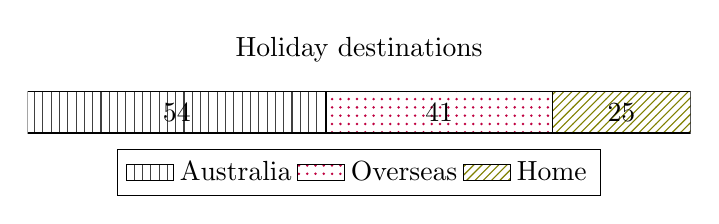
\begin{tikzpicture}
    \begin{axis}[
        xbar stacked,
        bar width=15pt,
        axis lines=none,
        xmin=0,
        xmax=120,
        height=2.2cm,
        width=10cm,
        title={Holiday destinations},
        enlarge y limits={abs=0.1},
        nodes near coords,
        legend style={at={(0.5,-0.1)}, anchor=north, legend columns=5, yshift=-1mm},
        legend image code/.code={
            \draw[#1] (0cm,-0.1cm) rectangle (0.6cm,0.1cm);
        },
        \mycyclelist
    ]
    \pgfplotsinvokeforeach{0,...,2}{
        \pgfmathparse{\mylegendlabels[#1]}
        \edef\tmp{\pgfmathresult}
        \pgfmathparse{\myxvalues[#1]}
        \edef\tmpx{\pgfmathresult}
        \addplot coordinates {(\tmpx,0)};
        \addlegendentryexpanded{\tmp};
    }
    \end{axis}
\end{tikzpicture}
\end{document}